{% -*- mode: LaTeX; TeX-PDF-mode: t; TeX-master: "manual"; -*-
}


\chapter{An Overview of the \ei Framework}
\label{ch:overview}

The \ei framework provides a simple way to build interfaces, e.g, a
web-interface or an Eclipse plugin, for tools written in (almost) any
programming language.
%
Moreover, it does not require the programmer to be familiar with any
GUI library or web programming. Roughly, the only requirement is that
the application can be executed from a command-line and that its
output goes to the standard output.
%
With the \ei framework we achieve the goal: \emph{build an application
  once, and get several sophisticated interfaces for free}.
%
In the rest of this chapter we explain the different components of
this framework, and how they are combined to achieve the above goal.
%
As will bed noticed later, the \ei framework was developed with
program analysis tools in mind, this why the graphical user interfaces
that it provides are basically developing environment that allow
editing programs, etc.

\section{The Architecture of \ei}
\label{ch:overview:arch}

\begin{figure}[h]
\begin{center}
\fbox{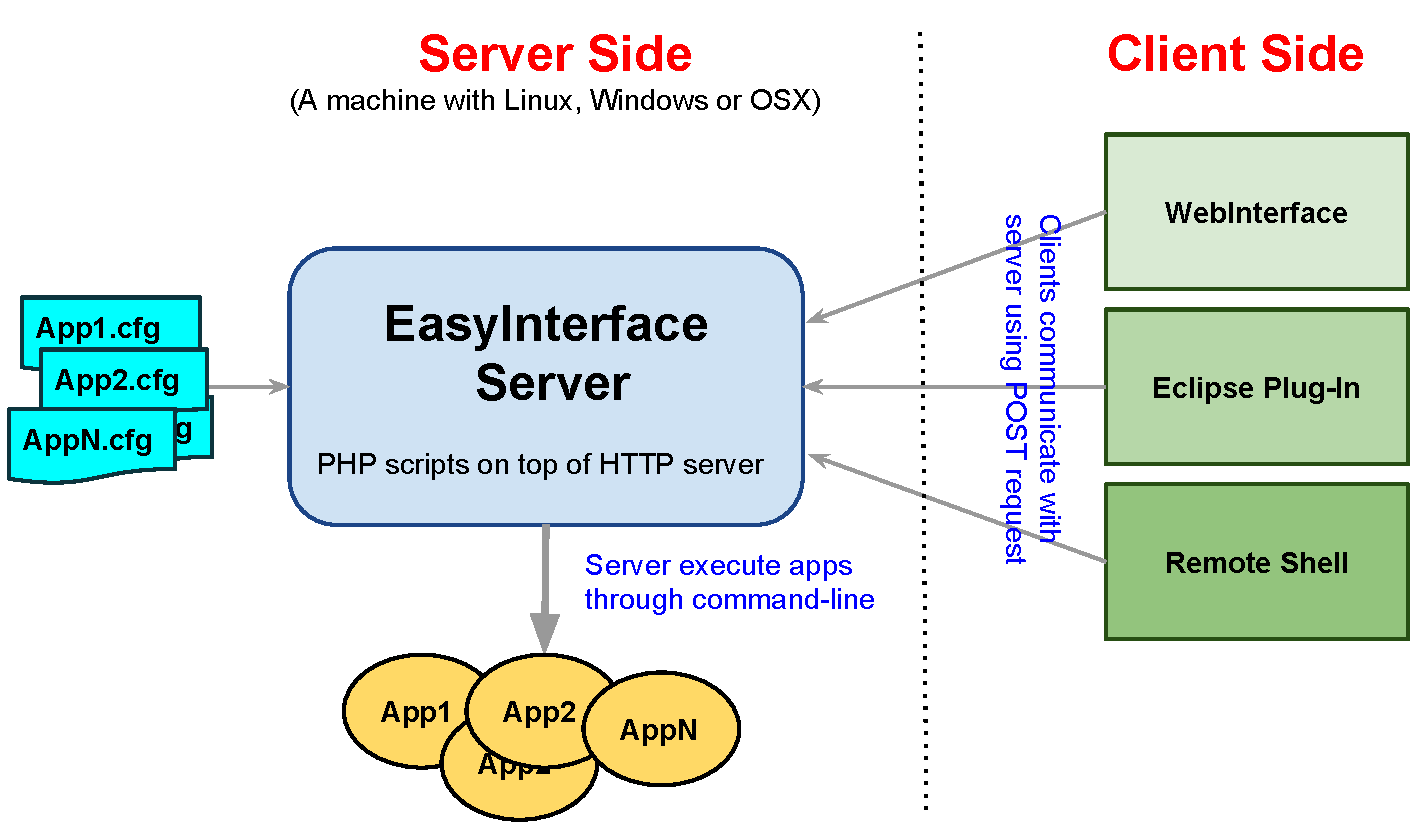
\includegraphics[width=0.5\textwidth]{fig/ei.pdf}}
\end{center}
\caption{The Architecture of the \ei Framework}
\label{fig:eiframework}
\end{figure}

The architecture of the \ei framework is depicted in
Figure~\ref{fig:eiframework}. It includes two main components:
%
(1) \emph{server side}: a machine with several applications (the
circles \texttt{App1}, \texttt{App2}, etc.) that can be executed from
a command-line and produce their output to the standard output. These
are the applications that we want to make available for the outside
world, i.e., execute them as services on the internet; and
%
(2) \emph{client side}: several clients that makes it easy to
  communicate with the server side to execute application, etc.
%
In what follows we start explaining the inner components of the server
side, and which problems they solve, and then we move on to explain the
client side.

\section{The Server Side}
\label{ch:overview:arch:server}

The problem that we want to solve at the server side is: 
%
\begin{quote}
  provide a uniform way for accessing the locally installed
  application as services (i.e., through the internet).
\end{quote}
%
This problem is solved by the \ei server, which is collection of PHP
programs that run on an HTTP server. The \ei server allows specifying
how a local applications can be executed and which parameter they take
using simple configuration files (\texttt{App1.cfg},
\texttt{App2.cfg}, etc.). For example, the following is a snippet of
such configuration file:

\medskip
\begin{lstlisting}
<app id='myapp' visible="true">
  ...
  <execinfo method="cmdline">
    <cmdlineapp>./default/myapp.sh _ei_parameters</cmdlineapp>
  </execinfo>
  <parameters prefix = "-" check="false">
    ...
    <selectone name="c">
      <option value="1" />
      <option value="2" />
    </selectone>
  </parameters>
</app>
\end{lstlisting}

\medskip
\noindent
This XML defines an application that has a unique identifier
\lst{myapp}.  The \lst{cmdlineapp} tag is a template that describes
how to execute the application from a command-line. Here
\lst{_ei_parameters} is a template parameter that will be replaced by
an appropriate value. The \lst{parameters} tag includes a list of
parameters accepted by the application. For example, there is a
parameter called ``\texttt{c}'' that can take one of the values $1$ or
$2$.
%
Once the configuration file is installed on the \ei server, anyone can
access the application using an HTTP POST request that include
something similar to the following:

\medskip
\begin{lstlisting}
{
  (*command: "execute",*)
  (*app\_id: "myapp",*)
  (*parameters:*) {
     (*c: ["1"],*)
     (*...*)
  },
  (*...*)
}
\end{lstlisting} 

\medskip
\noindent
When the \ei server receives such a request, it generates a
corresponding command-line (according to what is describe din the
configuration file), executes it, and redirect the standard output
back to the client.

\section{The Clients Side}
\label{ch:overview:arch:clients}

Although we now have a relatively easy way to execute applications on
the server side, it is still not as easy as we aimed at.
%
Our aim is to simplify this process further by providing (graphical)
user interfaces that automatically (1) connect to the \ei server and
ask for the list of available applications; (2) let the user choose an
application to execute and set the values of the corresponding
parameters; (3) generate a corresponding request and send it to the
\ei server; and (4) shows the returned output to the user.
%
The \ei framework provides three such interfaces: a
\emph{web-interface} that can be executed in a browser and looks like
a developing environment; an Eclipse-plugin that runs within the
Eclipse IDE; and a remote-shell that can be used from a command-line.

Since the web-client and the Eclipse plugin include are GUI based
developing environments, \ei provide also, to an application, the
possibility to generate output that has some graphical effect, e.g.,
open dialog-boxes, highlight code line, add markers, etc. To use this
feature, the applications should be modified to use the \ei output
language. The following is a snippet of such output:

\medskip
\begin{lstlisting}
<highlightlines dest="/Examples_1/iterative/sum.s"> 
  <lines> <line from="5" to="10"/> </lines>
</highlightlines>
...
<oncodelineclick dest="/Examples_1/iterative/sum.c" outclass="info" >
  <lines><line from="17" /></lines>
  <eicommands>
    <dialogbox boxtitle="Hey!"> 
      <content format="text">
       (* Click on the marker again to close this window *)
      </content>
    </dialogbox>
  </eicommands>
</oncodelineclick>

\end{lstlisting}

\medskip
\noindent
The \lst{highlightlines} indicates that lines $5--10$ of the file
\texttt{/Examples\_1/iterative/sum.s} (which is opened in the editor)
should be highlighted. The \lst{oncodelineclick} tag indicates that
when clicking on line $17$, a dialog-box with a corresponding message
should be opened.
%
Note that the application is only modified once to produce such
output, then it will have a corresponding effect in all interfaces
that support this language.





%%% Local Variables: 
%%% mode: latex
%%% TeX-master: "manual"
%%% End: 
